%%% Local Variables:
%%% mode: latex
%%% TeX-master: "../doc"
%%% coding: utf-8
%%% End:
% !TEX TS-program = pdflatexmk
% !TEX encoding = UTF-8 Unicode
% !TEX root = ../doc.tex

This section shows the results achieved during realization of the project.

\subsection{Overview PlanProject vs TogglProject} \label{Graphical overview}
To display the difference between the plan projects and the corresponding Toggl project, three different charts are displayed in the charts tab.
\begin{itemize}
	\item Total overview
	\item Projects overview
	\item Project time range overview
\end{itemize}
The different charts are explained in more detail in the following subsections.

\subsubsection{Total Overview}
This bar chart shows the overall sum of the time planned for all plan projects, compared to the total tracked time of their associated Toggl projects. Additionally, a prediction of how much time will be needed according to the future plan entries is displayed. An example for two projects is shown in \ref{figure9}.
\begin{figure}[H]
	\centering
	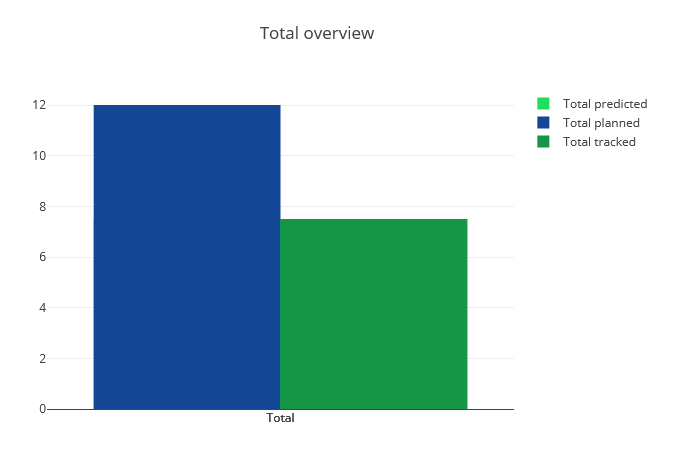
\includegraphics[width=1.0\columnwidth]{TotalOverview}
	\caption{Total Overview}
	\label{figure9}
\end{figure}

\subsubsection{Projects Overview}
This bar chart is similar to the total overview, but the single projects are displayed separately. An other minor difference is that the prognosis is added to both the tracked time and the planned time, creating a prediction for both. An example for two projects is shown in \ref{figure10}.
\begin{figure}[H]
	\centering
	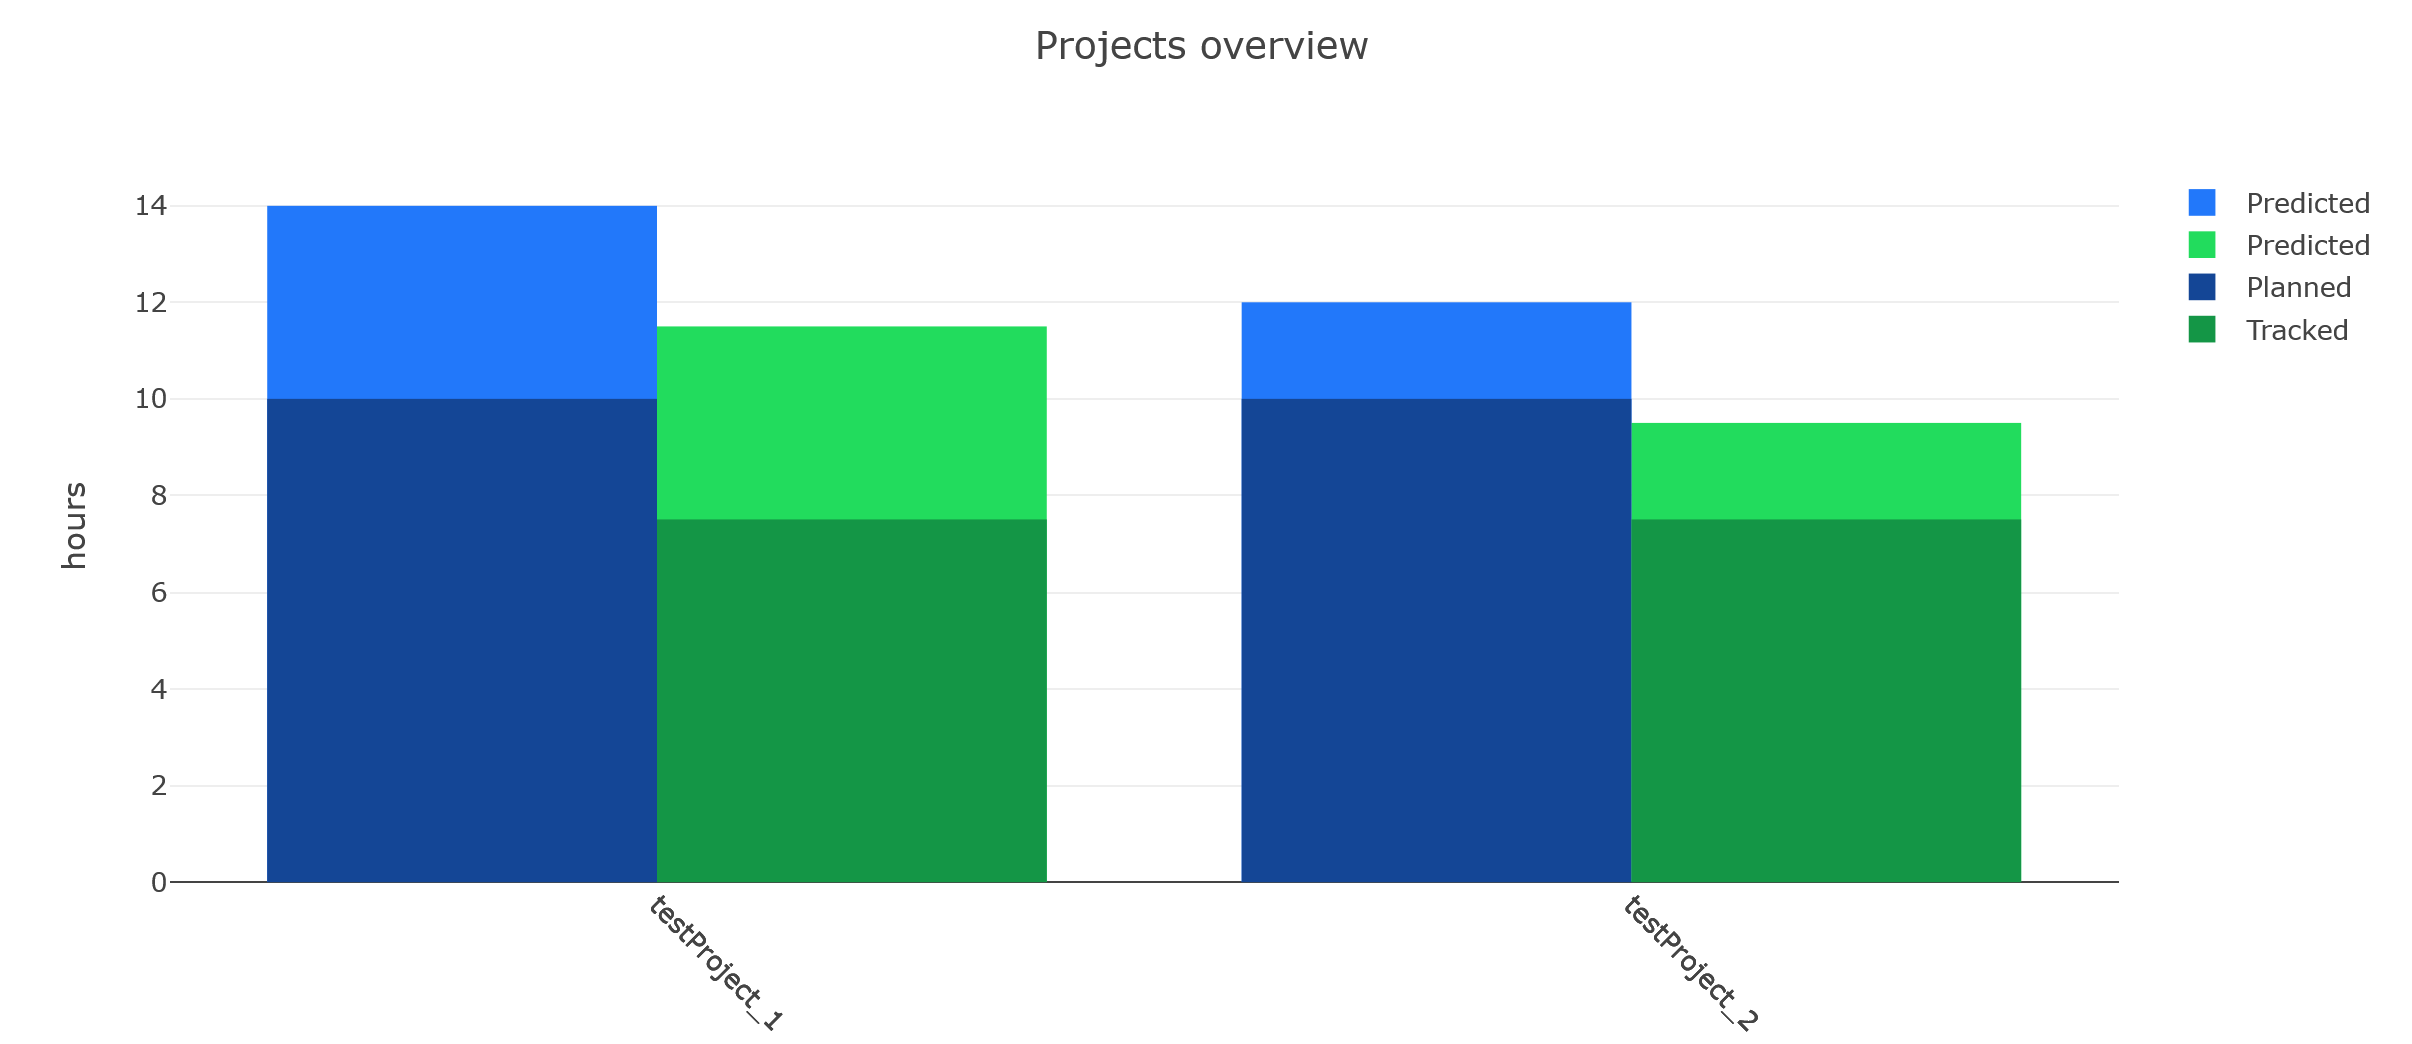
\includegraphics[width=1.0\columnwidth]{ProjectOverview}
	\caption{Total Overview}
	\label{figure10}
\end{figure}

\subsubsection{Project time range overview}
To display the chart, the user first has to choose the applicable time range. On hitting the "Filter setzen" button, the time range is set, and a line chart is drawn for every project, showing the development of planned time and tracked time during the selected time range. To reset the filter, the "Filter neu setzen" button has to be hit. This chart allows to see how the time amounts displayed in the other charts have been achieved and thus allows a user to estimate the quality of their planning. An example for one project is shown in \ref{figure11}.
\begin{figure}[H]
	\centering
	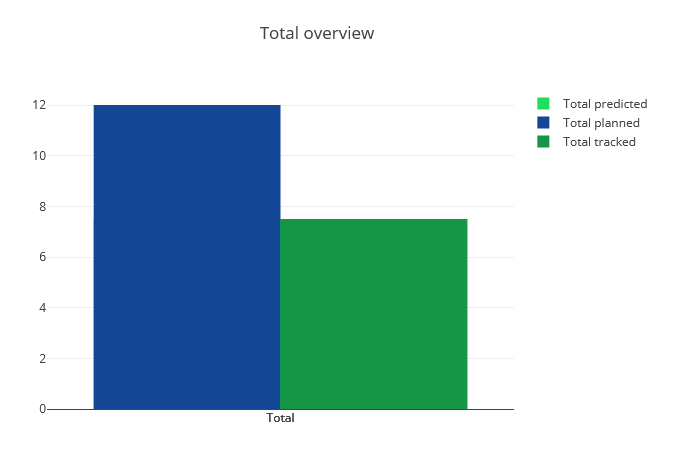
\includegraphics[width=1.0\columnwidth]{TimeOverview}
	\caption{Time Overview}
	\label{figure11}
\end{figure}